\documentclass[crop,tikz]{standalone}
\usetikzlibrary{backgrounds}
\colorlet{blue}{cyan}
\tikzset{
  inverted/.style = {
    every path/.style = {draw=white,text=white},
    background rectangle/.style={fill},
    show background rectangle
  }
}

\tikzset{>=latex}
\usetikzlibrary{calc}

% Centered arc
% Syntax: [draw options] (center) (initial angle:final angle:radius)
\def\centerarc[#1](#2)(#3:#4:#5);%
{
  \draw[#1]([shift=(#3:#5)]#2) arc (#3:#4:#5);
}

\begin{document}
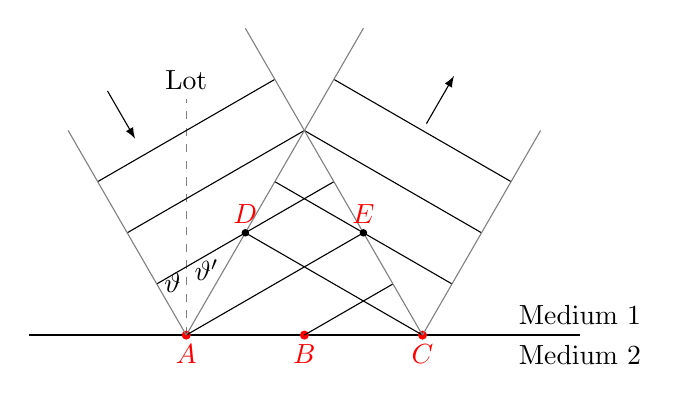
\begin{tikzpicture}
  \coordinate (a) at (1,0);
  \coordinate (b) at (2.5,0);
  \coordinate (c) at (4,0);
  % boundary
  \draw[thick] (-1,0) -- +(7,0) node[above] {Medium $1$} node[below] {Medium $2$};
  % plumb
  \draw[gray,dashed] (a) -- +(0,3) node[above,black] {Lot};
  \centerarc[gray](a)(90:120:1);
  \node[below] at ($(a)+(100:1)+(0,-0.08)$) {$\vartheta$};
  \centerarc[gray](a)(60:90:1.2);
  \node[below] at ($(a)+(80:1.2)+(0.05,-0.1)$) {$\vartheta'$};
  % elementary wave
  \draw[fill,red] (a) circle (0.05) node[below] {$A$};
  \centerarc[blue](a)(180:0:0.5*3);
  % elementary wave
  \draw[fill,red] (b) circle (0.05) node[below] {$B$};
  \centerarc[blue](b)(180:0:0.5*1.5);
  % elementary wave
  \draw[fill,red] (c) circle (0.05) node[below] {$C$};
  % wave fronts
  \draw[] (a) -- +(30:0.866*3);
  \draw[] (b) -- +(30:0.866*1.5);
  \foreach \X in {1,2,3} { \draw ($(a)+(120:0.5*1.5*\X)$) -- +(30:0.866*3); };
  \foreach \X in {0,1,2,3} { \draw ($(c)+(60:0.5*1.5*\X)$) -- +(150:0.866*3); };
  % boundary
  \draw[gray] (a) -- +(120:3);
  \draw[gray] (a) -- +(60:3+0.5*3);
  \draw[gray] (c) -- +(120:3+0.5*3);
  \draw[gray] (c) -- +(60:3+0);
  % arrows
  \draw[->] (0,3.1) -- +(-60:0.7);
  \draw[->] ($(b)+(60:3.1)$) -- +(60:0.7);
  % points
  \coordinate (d) at ($(c)+(150:0.866*3)$);
  \coordinate (e) at ($(a)+(30:0.866*3)$);
  \draw[fill] (d) circle (0.04);
  \draw[fill] (e) circle (0.04);
  \node[above,red] at (d) {$D$};
  \node[above,red] at (e) {$E$};
\end{tikzpicture}
\end{document}
